%
% main.tex -- Paper zum Thema gis
%
% (c) 2019 Hochschule Rapperswil
%
\chapter{Signalanalyse von UHF Teilentladungssignalen im Zeitbereich \label{chapter:gis}}
\lhead{Signalanalyse von UHF Teilentladungssignale im Zeitbereich}
\begin{refsection}
\chapterauthor{Kris Wyss}

\section{Gasisolierte Schaltanlagen}
\rhead{Vorwort}

Gasisolierte Schaltanlagen (GIS) dienen der elektrischen Energieverteilung, dem Schutz der Komponenten und ermöglichen eine sichere Wartung des Energieübertragungsnetzes.
Als Isoliergas wird Schwefelhexafluorid (SF\textsubscript{6}) eingesetzt. SF\textsubscript{6} hat bei Atmosphärendruck eine etwa drei mal so grosse dielektrische Festigkeit (Spannungs-Isolationsvermögen) wie Luft. 
Es besitzt auch um den Faktor 3 bis 4 mal bessere Lichtbogenlöscheingeschaft als Luft. 
Diese Eigenschaften führen zu einer erheblichen Platzeinsparung gegenüber einer luftisolierten Schaltanlage (AIS) \cite{buch:ABB}.
Deshalb und wegen einigen anderen Gründen, aufgezeigt in \cite{buch:GIS/AIS}, hat sich der Einsatz von GIS überall dort durchgesetzt wo Boden teuer ist. Zum Beispiel in urbanen Gebieten. Aber auch bei luftisolierten Schaltanlagen ab 72.5 kV sind die Leistungsschalter mit SF\textsubscript{6} befüllt. 
Bei Leistungsschaltern dient das SF\textsubscript{6} als Löschgas des Lichtbogens, welcher bis zu mehreren tausend Ampere trägt, wenn ein Teil des Übertragungsnetzes von der Last freigeschaltet  wird \cite{buch:ABB}.

Bei der Quantifizierung der Qualität einer GIS spielt der Begriff Teilentladung (TE) eine wichtige Rolle. 
Wenn das E-Feld örtlich über die dielektrische Festigkeit steigt entstehen elektrische Entladungen, welche nur ein Teil der Isolationsstrecke überbrücken und nicht zu einem kompletten Durchschlag führen, daher die Namensgebung Teilentladung \cite{buch:Kuchler}.
Teilentladung im Isolierstoff lässt das Isoliermedium  schneller altern. Dies kann zum dielektrischen Durchschlag führen welcher einen Totalausfall der Anlage zur folge hat.
Aufgrund dessen ist TE ein wichtiges Qualitätsmerkmal bei Hochspannungskomponenten. 

Tritt Teilentladung auf werden verschiedene  physikalische Prozesse initiiert. 
Die Entladung hat einen Strompuls zur Folge.
Wegen dem Lichtbogen wird eine ultrahochfrequente (UHF) elektromagnetische Welle emittiert.
Die schnellste gemessene Anstiegszeit des Strompulses in SF\textsubscript{6} liegt bei 24ps.
Dies entspricht einem Frequenzband hoch bis zu 14 GHz \cite{skript:Judd24ps} . 
Aufgrund der schnellen Erhitzung des Gases rund um den Lichtbogen wird danach eine Schallwelle abgestrahlt. 
Ebenfalls durch die grosse Erhitzung wird das Isoliergas SF\textsubscript{6} zersetzt. 
Somit kann TE chemisch, akustisch oder elektromagnetisch gemessen und lokalisiert werden \cite{skript:StatusReviewPDMeasurement}.
In dieser Arbeit wird auf die Analyse der UHF TE-Signale eingegangen.
Es wird versucht, mittels dem Signalanalyseverfahren kontinuierliche Wavelettransformation (CWT), fehlerspezifische Charakteristiken im Zeitsignal der elektromagnetischen Welle auszumachen.

\section{Fehlerarten und Analyse in GIS}
\rhead{Abschnitt}

TE wird in zwei Grundkategorien unterteilt \cite{buch:Kuchler}, die Innere- und Äussere-TE. 
Die Erstere ist dadurch charakterisiert das sich die TE-Quelle im Innern eines festen oder flüssigen Isolierstoffes befindet. 
Spezifiziert auf GIS gehören zu Kategorie der Inneren-TE Lunker, Risse/Spalten in Isolierstoffe und Delamination zwischen Isolierschichten.
 
Entladungen an äusseren Leiterstrukturen wird als Äussere-TE oder Korona bezeichnet. 
In GIS kommen folgende Fehler aus dieser Kategorie vor, Oberflächenentladung und Koronaentladung. 
Oberflächenentladungen treten bei nicht Einhalten der Herstellungstoleranzen zwischen leitendem und isolierendem Material auf.
Eine weitere Quelle sind potenzialfrei leitende Partikel auf festen Isolierstoffen.
Spitzen und scharfe Kanten an spannungsführenden- und an leitfähigen-Teilen auf Erdpotenzial führen zu Koronaentladung \cite{buch:Kuchler, skript:AeussreTE, skript:InnereTE}. 
In dieser Arbeit werden UHF TE-Signale von Oberflächenentladung und Hohlraumentladungen analysiert. 
Im weiteren Abschnitt werfen wir einen genaueren physikalischen Blick, auf die zwei Entladungsarten und die herkömmliche Fehleranalyse.

\subsection{Oberflächenentladung}

Diese Entladungsart entsteht, wenn an Oberflächen von Festisolierstoffen hohe elektrische Feldstärken auftreten. 
Dies kann konstruktionsbedingt oder Aufgrund von unsauberer Montage entstehen.
Wenn sich ein Braue oberhalb eines Festisolierstoffes befindet oder ein loser metallischer Partikel auf einem Isolierstoff ist, dann entladen sich die Stromimpulse über das Isoliermaterial. 
In Abbildung \ref{fig:oberflaechenentladung} ist schön ersichtlich das die Art der TE einer Koronaentladung entspricht. Jedoch verteilen sich die Elektronen nicht im Gasraum sondern sie gleiten über die Isolierfläche (helle Fläche).
\begin{figure}
	\centering
	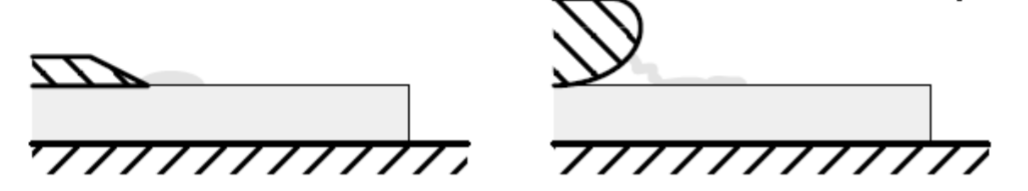
\includegraphics[width=0.7\linewidth]{papers/gis/Bilder/Oberflaechenentladung}
	\caption{Zwei Anordnungen von Oberflächenentladungen \cite{buch:Kuchler}}
	\label{fig:oberflaechenentladung}
\end{figure}
Das Ersatzschaltbild (ESB) \ref{fig:M1} besteht aus einer Kapazität C parallel zu einer Funkenstrecke F und einem Widerstand R in Serie. 
Der Pfeil steht für die Spitze an welcher ein inhomogenes elektrisches Feld ansteht.
Wenn das inhomogene elektrische Feld über der Kapazität C einen kritischen Wert überschreitet entlädt sich die gespeicherte Energie über die Funkenstrecke F gegen Erde.
Dies kann bei Wechselspannung 50Hz mehrmals pro Halbwelle geschehen \cite{skript:AeussreTE}. 
\begin{figure}
\centering
\begin{circuitikz} [scale=0.6] \draw
(0,1)node[vee]{Spitze} (0,1)--(0,0)
to[C=$C$] (0,-3)
to[R=$R$]  (0,-5)
node[rground]{}
(0, 0) -- (3, 0.0) -- (3, -1) 
to[american gas filled surge arrester=$F$] (3, -2) -- (3, -3) -- (0,-3)
	;
\end{circuitikz}
\caption{ESB: Koronaentladung} \label{fig:M1}
\end{figure}


\subsection{Hohlraumentladung}

Die häufigste Form von Hohlraumentladungen in GIS ist aufgrund von Hohlräumen/Lunkern im Isolierstoff. 
Hohlräume entstehen beim Herstellungsprozess der Isolatoren. Während dem Abkühlprozess kann es zu Diffusionsvorgänge in der
Isoliermasse kommen, dadurch können sich gasgefüllte Hohlräume im Isolierstoff ausbilden. 
Oft geht man im Model von runden, luftgefüllten Hohlräumen mit niedriger elektrischer Festigkeit aus. 
Jedoch sind in der Praxis die genauen geometrischen und dielektrischen Eigenschaften nicht bekannt da die Fehlstelle nicht zugänglich ist. 
In Abbildung \ref{fig:hohlraum} sind diverse Hohlräume 1--3 illustriert. Unter der Nummer 1 sind klassische runde oder ellipsenförmige Lunker ohne Elektrodenkontakt abgebildet. 
Die beiden anderen Hohlräume haben Elektrodenkontakt und die Nummer 3 stellt eine Ablösung von der Leitfähigen Elektrodenschicht dar  \cite{buch:Kuchler, skript:InnereTE}.

Elektrisch wird die Fehlerart mit dem Ersatzschaltbild gemäss \ref{fig:M2} modelliert. 
Die Kapazität C\textsubscript{0} stellt dabei die Gesamtkapazität über die Isolierstrecke dar und C\textsubscript{h} ist die Hohlraumkapazität welche die Fehlerstelle abbildet.
Die Spannung $u_{h}(t)$ folgt der äusseren Spannung $u(t)$ bis die Zündspannung erreicht ist. 
Bei dieser Spannung hat die Feldstärke über der Hohlraumkapazität einen kritischen Wert überschritten und die Energie, bei vorhanden sein eines Startelektrons, entlädt sich über die Funkenstrecke F.
Die Spannung über $u{h}(t)$ sinkt bis zur Löschspannung, danach kann sich der selbe Vorgang mehrere Male pro Halbwelle wiederholen. 
Über die Serienkapazität C\textsubscript{s} wird die Hohlraumkapazität C\textsubscript{h} via einen kapazitiven Verbschiebestrom nachgeladen \cite{buch:Kuchler}. 

\begin{figure}
	\centering
	\begin{circuitikz} [european, scale=0.5] 
		\draw
		(-3,0)node[vcc]{Hochspannung} (-3,0)--(-3,-1)
		to[C=$C_0$] (-3,-3) -- (-3,-4)
		node[rground] {}
		(-3.5, 0) to[open, v=$u(t)$] (-3.5, -4)
		
		(0,0)
		to[C=$C_s$] (0,-2) 
		to[C=$C_h$, v=$u_h(t)$] (0,-4)
		node[rground]{}
		
		(-3,0) --(0, 0)
		
		(0, -2) -- (3,-2) to[american gas filled surge arrester=$F$] (3, -4)
		node[rground]{} 
		;
	\end{circuitikz}
	\caption{ESB: Hohlraumentladung} 
	\label{fig:M2}
	\end{figure}

\begin{figure}
	\centering
	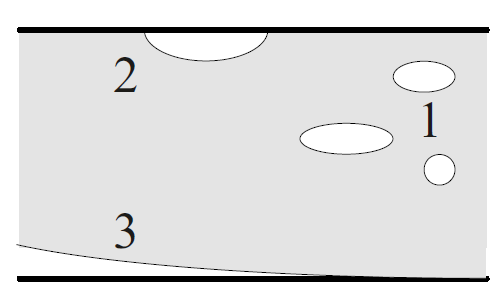
\includegraphics[width=0.5\linewidth]{papers/gis/Bilder/Hohlraum}
	\caption[]{Bsp. von geometrisch verschiedenen Hohlräume mit und ohne Elektrodenkontakt \cite{buch:Kuchler}}
	\label{fig:hohlraum}
\end{figure}
  
\subsection{Herkömmliche Fehleranalyse}

Um die fehlerspezifischen physikalisch und elektrotechnischen Phänomene bildlich darstellen zu können muss ein Bezug hergestellt werden zwischen dem Entladungszeitpunkt und dem Phasenwinkel der Hochspannung, welche am Prüfling anliegt. 
Mit diesen Daten wird ein phasenaufgelöstes Teilentladungsmuster (PRPD: Phase-resolved partial discharge) erstellt. 
In dem Bild wird die Korrelation zwischen der Phasenlage $\phi$, Amplitudenhöhe $Q$ und der Anzahl Entladungen $N$ gemacht \cite{buch:UHFSignale}. 
In Abbildung \ref{fig:PRPDAlg} sind diese Zusammenhänge aufgezeigt und in Abbildung \ref{fig:PRPDHohl} 
ist ein Beispiel. dargestellt wie das Muster einer typischen Oberflächenentladung aussieht. 
Im oberen Bereich ist die Phasenlage der angelegten Spannung aufgezeigt und im unteren Bildteil sind die Entladungen gemäss dem in Abbildung \ref{fig:PRPDAlg} gezeigten Algorithmus ersichtlich.
Die Muster werden über den Zeitraum von einer bis mehreren Minuten aufgezeichnet.
\begin{figure}
	\centering
	\begin{minipage}{.5\textwidth}
		\centering
		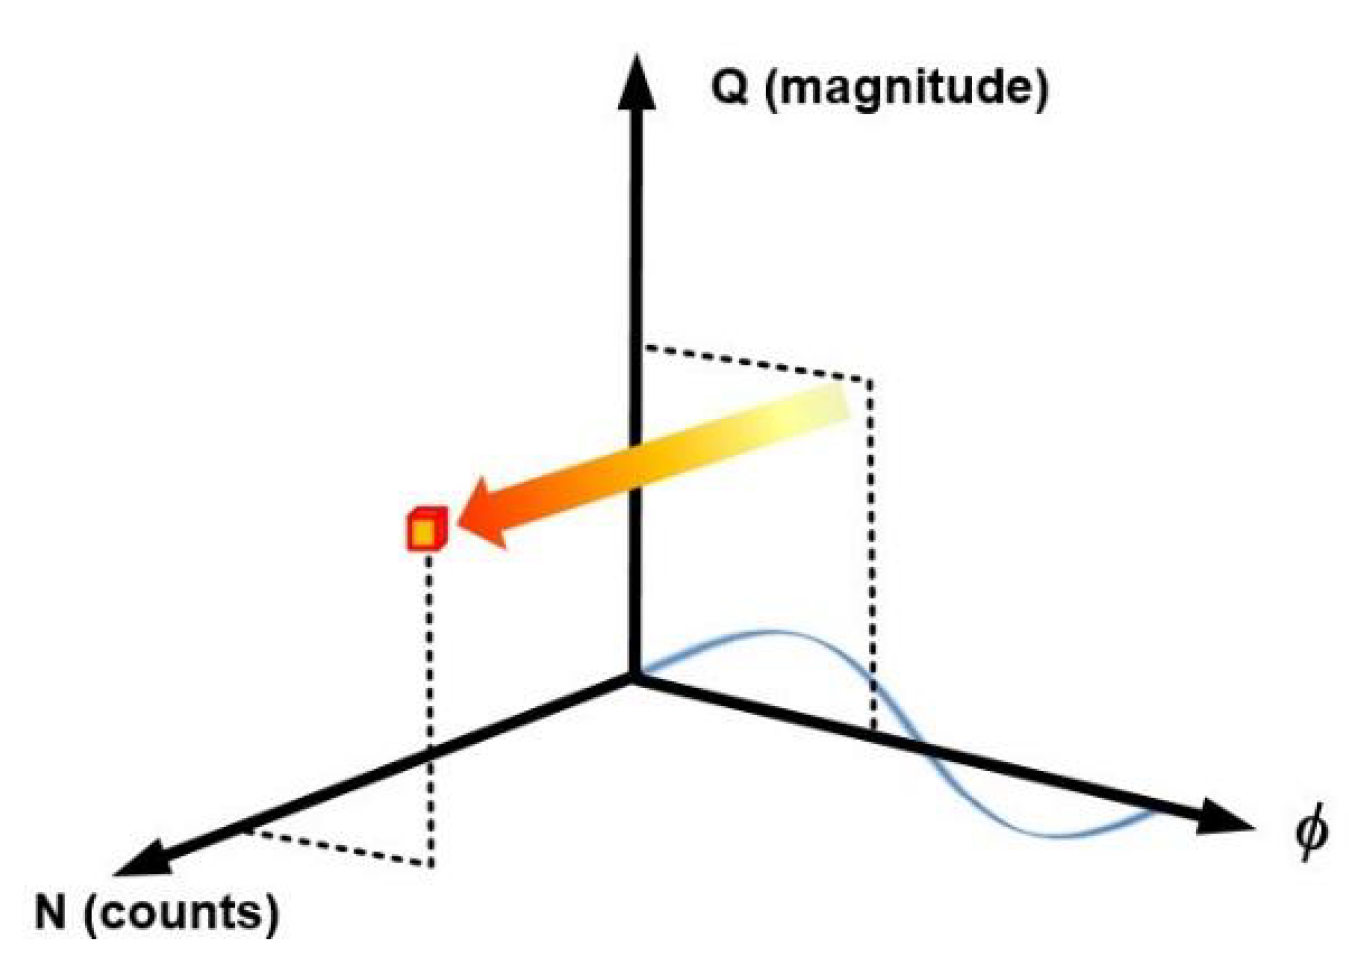
\includegraphics[width=.9\linewidth]{papers/gis/Bilder/PERP}
		\captionof{figure}{PRPD Algorithums \cite{report:ABBOnSite}}
		\label{fig:PRPDAlg}
	\end{minipage}%
	\begin{minipage}{.5\textwidth}
		\centering
		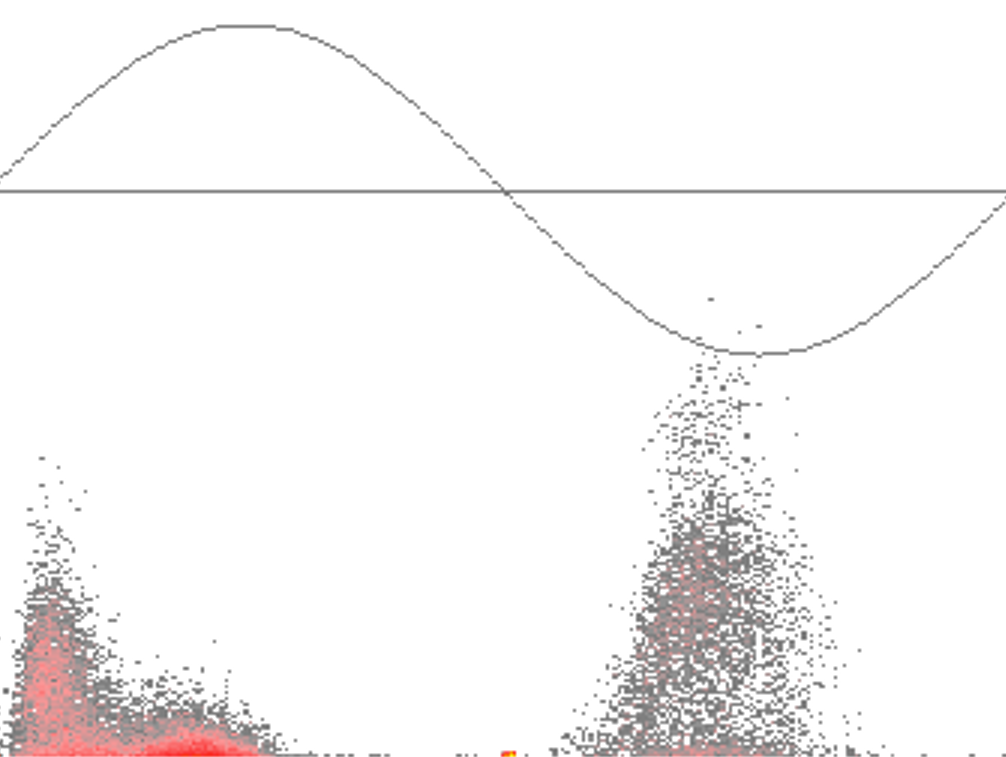
\includegraphics[width=.8\linewidth]{papers/gis/Bilder/OberflaechenentladungPRPD}
		\captionof{figure}{Typisches PRPD-Muster}
		\label{fig:PRPDHohl}
	\end{minipage}
\end{figure}


\section{Messpfad}
\rhead{Abschnitt}
In diesem Bericht wird untersucht, ob mit der kontinuierlichen Wavelet Transformation fehlerspezifische Merkmale im Zeitsignal auszumachen sind. 
Dafür ist es wichtig das wir den Messpfad von der Fehlerursache bis zum Oszilloskop kennen. 
Die untersuchten Signale wurden bei einer Vor-Ort Abklärung, an einer Anlage die im Betrieb war, aufgezeichnet.  
Im ersten Abschnitt wird auf den Signalpfad innerhalb der GIS eingegangen und in einem zweiten auf die Messkette ausserhalb.

Bei der Fehlstelle [0] wird Aufgrund der schnellen Entladung eine elektromagnetische  Welle vom Strompuls abgestrahlt. 
Die Welle besitzt Frequenzanteile bis in den zweistelligen GHz Bereich. 
In erster Annäherung wird die GIS oft als Koaxialkabel modelliert. 
Diese Vereinfachung ist jedoch nicht ausreichend da Reflexionsphänomene auftreten. 
Aufgrund von diversen Unstetigkeitsstellen in einer GIS, wie z.B Stützisolatoren [1], Verzweigungen [2],  Änderung der Leiterdurchmesser [3], schaltende Elemente und die Enden der Anordnung, ändert der Wellenwiderstand und es kommt zu Reflexionen der Welle.
Durch diese entstehen stehende Wellen in der GIS und die Signalleistung wird gedämpft. 
In Abbildung \ref{fig:messketteingis} sind einige approximative Dämpfungswerte angezeigt \cite{report:PDBasicABB}.
Eine GIS im Feld hat an diversen Stellen breitbandige Sensoren [4] die wie Antennen wirken. 
An diesen kann das Signal aus der GIS gekoppelt werden. \cite{buch:UHFSignale, skript:Judd24ps, buch:Kuchler} 
\begin{figure}
	\centering
	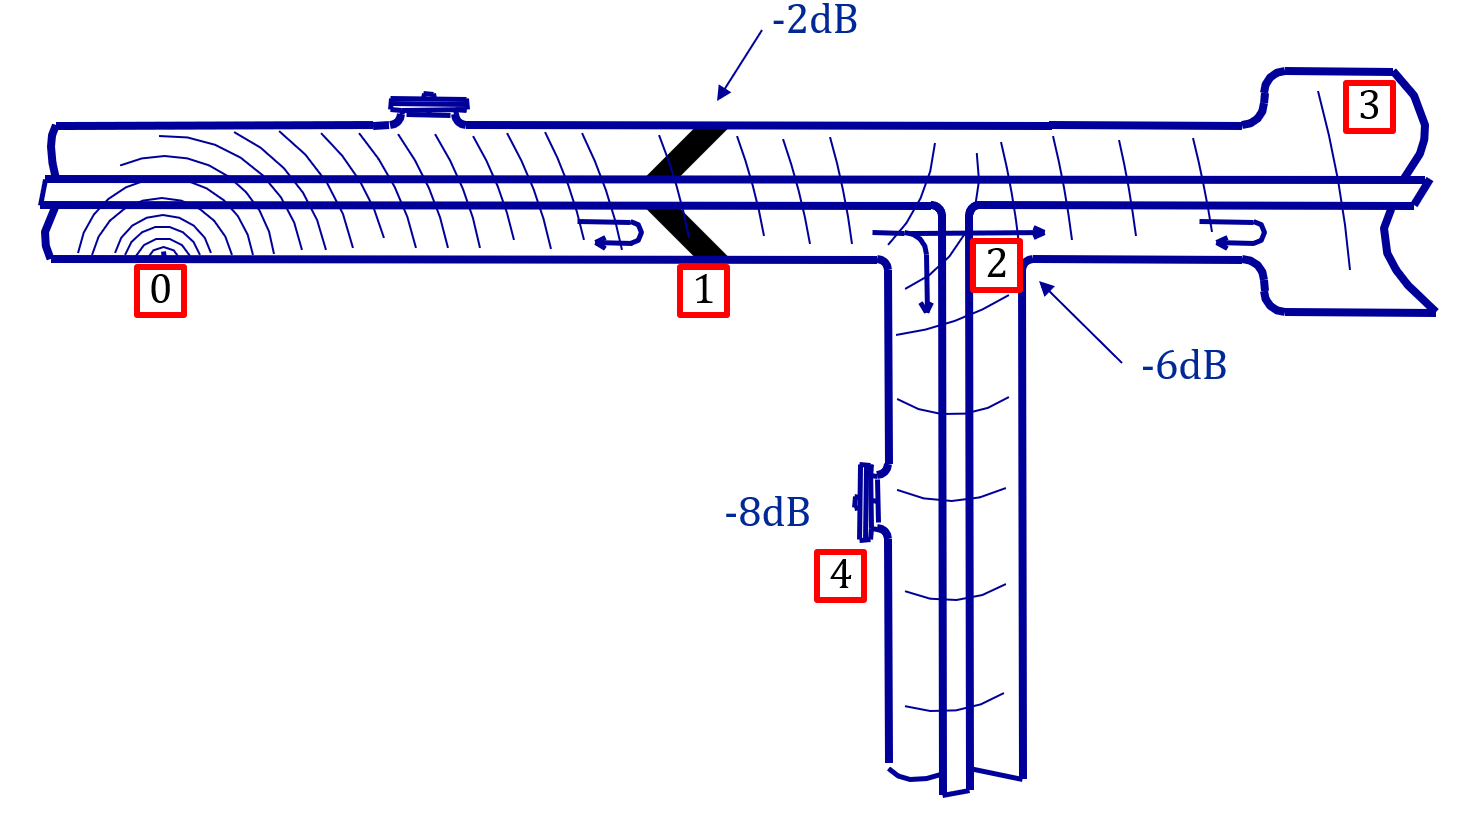
\includegraphics[width=0.5\linewidth]{papers/gis/Bilder/MessketteInGIS}
	\caption{Unstetigkeitsstellen GIS \cite{report:PDBasicABB}}
	\label{fig:messketteingis}
\end{figure}

Nach dem Sensor ist ein Hochpassfilter mit der Eckfrequenz 83MHz vorgeschaltet.
Dieser dient zum Schutz der dahinterliegenden Messgeräte.
Falls es zu einem dielektrischen Durchschlag kommt werden die hochenergetischen Signalanteile gegen Erde abgeleitet.
Danach wird das Signal mit 50dB verstärkt.
Die 50$\Omega$ Signalkabel werden an einen Multiplexer gehenkt. 
Mit dem kann das Signal auf einem Frequenzanalysator oder Oszilloskop angezeigt werden. 
Für die untersuchten Daten sind die Zeitsignale mit einem 10GS/s Oszilloskop mit 2GHz Bandbreite aufgezeichnet worden.
Die Abtastzeit wurde für alle Signale gleich gewählt und liegt bei 100ps. 
\begin{figure}
	\centering
	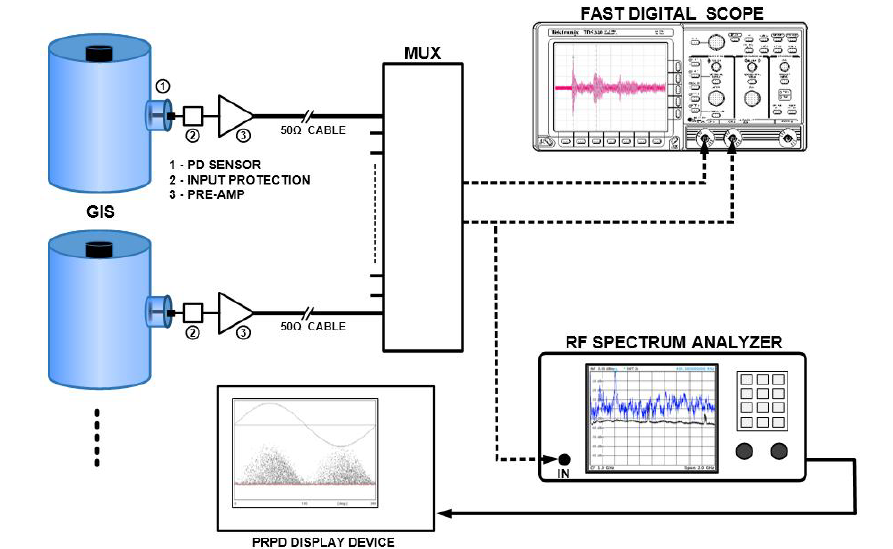
\includegraphics[width=0.5\linewidth]{papers/gis/Bilder/MessketteAusGIS}
	\caption{Messkette \cite{report:ABBOnSite}}
	\label{fig:messketteausgis}
\end{figure}

 
\section{Datenbearbeitung}
\rhead{Abschnitt}

Die Zeitsignale welche untersucht wurden sind aufgenommen worden bei Laufzeitmessungen (TOF: Time of flight). 
Bei einer TOF Messung sind nur die Anfänge der Signale von -interesse.
Dies Bedeutet das selten die ganze Einhüllende aufgezeichnet wird und oft werden die Analog Digital Wander (ADC) übersteuert. 
Somit sind die Signale nicht brauchbar für eine CWT.
Es wurden aus ca. 700 Aufzeichnungen vier passende Signale gefunden wo fast komplett abklingen und die Signalamplituden korrekt aufgezeichnet sind. 
Mit Hilfe des Kundenberichtes welcher die PRPD Muster enthält und den Handnotizen wo die Zeitstempel und Ortsangaben vermerkt sind, konnten die Zeitsignale den Fehlerquellen zugeordnet werden.
Es sind je zwei Exemplare von Hohlraumentladung und Oberflächenentladung.
\begin{figure}
	\centering
	
	\begin{subfigure}
		\centering
		\begin{tikzpicture}
		\begin{axis}
		[
		title = a),
		width = 10cm,
		height = 3.5cm,
		xmin = -1.5e-7,
		xmax = 0.8e-6,
		xlabel=time (s),
		ylabel=voltage (V)
		]
		\addplot [red] coordinates{(-1.5e-7, 0.03) (8e-7, 0.03)};
		\addplot [black, samples=10000] file {papers/gis/Messdaten/Data.txt};
		\node[pin=145:{Start}] at (axis cs:0,0) {};
		\node[pin=155:{Treshold}] at (axis cs:6e-7,0.03) {};
		\end{axis}
		\end{tikzpicture}
	\end{subfigure}
	\begin{subfigure}
		\centering
		\begin{tikzpicture}
		
		\begin{axis}
		[
		title = b),
		width = 10cm,
		height = 3.5cm,
		xmin = -0.15e-7,
		xmax = 3e-7,
		xlabel=time (s),
		ylabel=voltage (V)
		]
		\addplot [black, samples=10000] file {papers/gis/Messdaten/Data.txt};
		\end{axis}
		\end{tikzpicture}
	\end{subfigure}	
\caption{a) Vor Harmonisierung b) Nach Harmonisierung}
\label{fig:Zeitsig}
\end{figure}

Damit die Messungen Sinnvoll miteinander vergleichbar sind, wurden einige Datenaufbereitungen im Matlabcode implementiert.
Dies dient zur Harmonisierung der zu untersuchenden Signale (siehe Abbildung \ref{fig:Zeitsig}). 
Auf diese wird im Folgenden kurz eingegangen.

Durch transformieren von vielen Signalen hat sich gezeigt, dass der interessante Bereich, wo die CWT relevante Muster hervorbringt, in den ersten 300ns ist.
Bei einer Abtastzeit von 100ps entspricht dies 3000 Datenpunkte.
Um den Startpunkt des Signals zu extrahieren wurde ein Treshholdlevel mit folgendem Algorithmus implementiert.
Aus den ersten 300 Datenwerte wird der Vektorindex $v_{max}$ mit dem grössten absolute Wert ermittelt.
Der Tresholdlevel wird durch quadrieren von Wert in $v_{max}$ und multiplikation mit 3 festgelegt.
\begin{equation}
Treshholdlevel = 3*v_{max}^2
\end{equation}
Der Startpunkt wird ermittelt in dem das erste Vektorelement im Datenvektor $abs(v_d)^2$ gesucht wird welches diesen überschreitet.
Dazu wird auch der gesamte Datenvektor quadriert.
Mit dem Quadrieren wird ein grösserer Signal-Rausch Abstand (SNR) erzielt.

Um die CWT Muster aussagekräftiger darzustellen wird auf der y-Achse nicht die Dilatationsskalierungen angezeigt. Stattdessen wird ein Rückschluss auf die Frequenz abgeleitet. Diese darf jedoch nur als Approximation betrachtet werden, da in einer CWT die Frequenzauflösung nicht der Auflösung einer Fourier-Transformation entspricht. Die Frequenzapproximation wird durch folgende Berechnung erreicht.
\begin{equation}
F_a=\dfrac{F_c}{a}
\end{equation}
Wobei $F_c$ der Mittelfrequenz des Wavelets entspricht.
Diese wird durch den höchsten Wert des Skalarproduktes 

\begin{equation}
F_c(t/a) = \max\langle x(t),y(t/a)\rangle
\end{equation}

zwischen dem Wavelet $x$ und dem Sinus $y$ berechnet.
Wobei der Sinus mit dem Dilatationsfaktor $a$ gestreckt wird.
In Abbildung \ref{fig:Mittenfrequ} ist die Mittenfrequenz von einem Daubechies-Wavelet Nr. 8 (db8) dargestellt.
Die Variable $a$ steht für den Dilatationsskalierungsfaktor. 
Damit wird erzielt das die y-Achse mit der approximierten Frequenz $F_a$ skaliert ist..

\begin{figure}
	\centering
	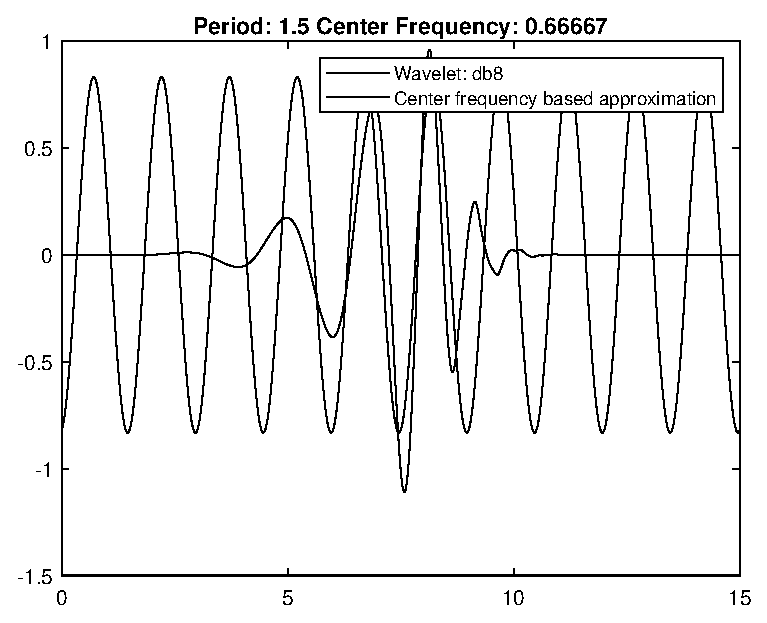
\includegraphics [width=0.7\linewidth] {papers/gis/Bilder/epsFig}
	\caption{Mittelfrequenzermittlung db8}
	\label{fig:Mittenfrequ}
\end{figure}


\section{Auswertung kontinuierliche Wavelettransformation}
\rhead{Abschnitt}

\section{Schlussfolgerung}
\rhead{Schlussfolgerung}
 
\printbibliography[heading=subbibliography]
\end{refsection}
